\chapter{Q-Learning, DQL, Reinforce, PPO}
\section{Q-Learning}
El algoritmo de Q-learning es una técnica de aprendizaje por refuerzo que permite a un agente aprender la política óptima para tomar decisiones en un entorno determinado.

Usa TD para actualizar la función acción-valor:
\begin{itemize}
    \item Actualiza las acciones-valores en cada interacción con el entorno.
    \item No aprende una política directamente, sino que la deriva de las acciones-valores de los estados (método basado en valor).
\end{itemize}



\begin{figure}[ht]
    \centering
    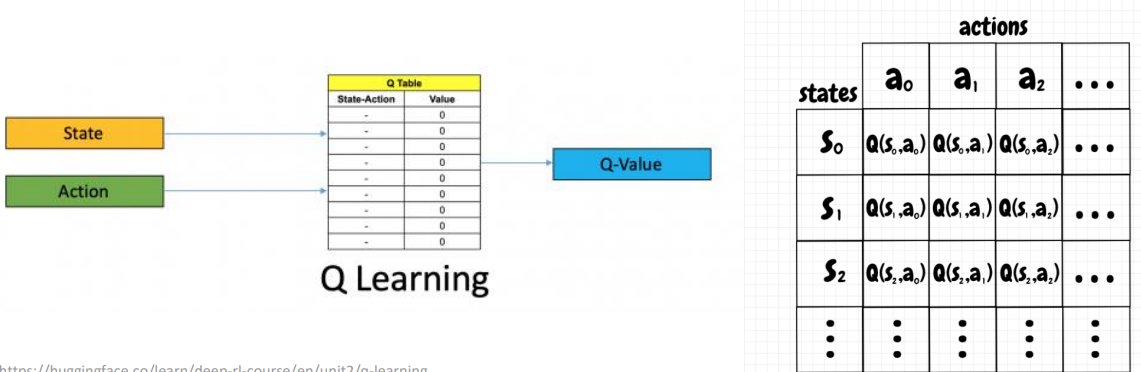
\includegraphics[width=0.75\linewidth]{imagenes/q-learning1.png}
    \label{fig:q-learning1}
\end{figure}



\begin{figure}[ht]
    \centering
    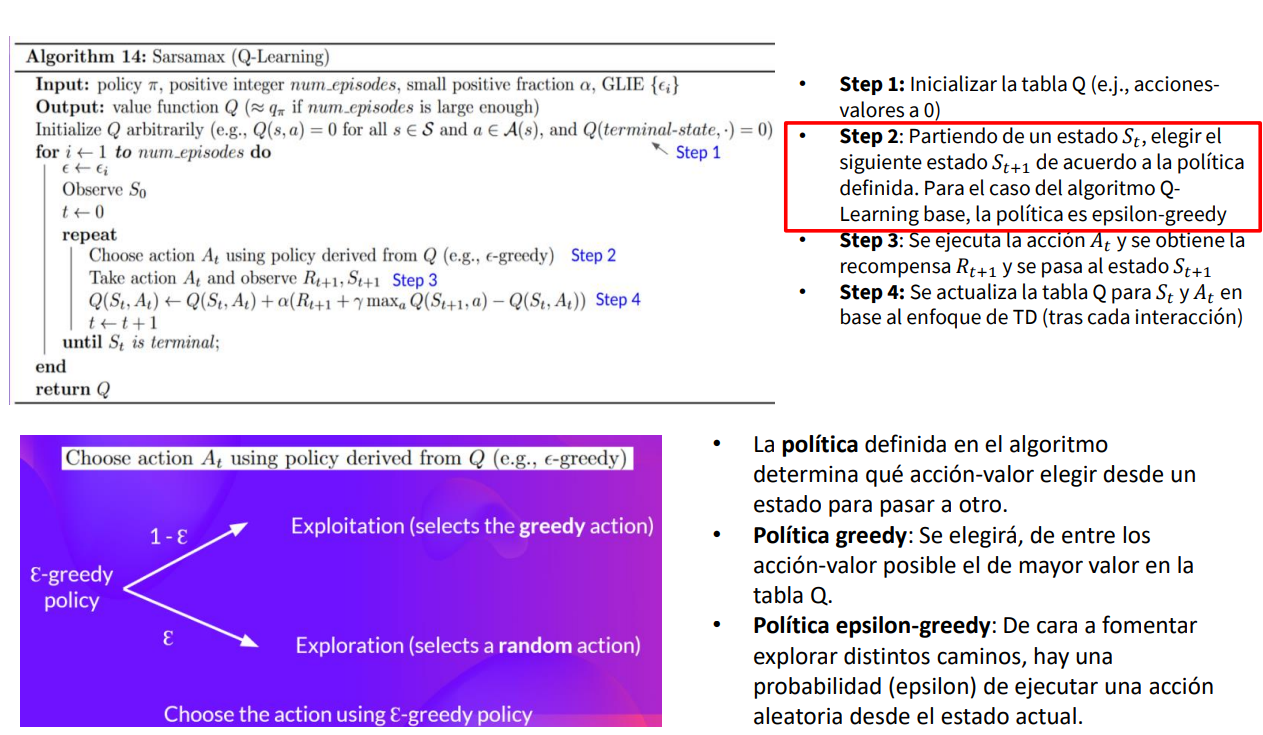
\includegraphics[width=0.75\linewidth]{imagenes/q-learning2.png}
    \label{fig:q-learning2}
\end{figure}


La fórmula de actualización se muestra en la siguiente ecuación:
\[
Q(s,a) \leftarrow Q(s,a) + \alpha \left[ r + \gamma \max_{a'} Q(s', a') - Q(s,a) \right]
\]

Donde:
\begin{itemize}
    \item $\alpha$ es la tasa de aprendizaje, que controla la actualización de los valores Q en cada paso ($0 < \alpha \leq 1$).
    \item $\gamma$ (gamma) es el factor de descuento, que determina la importancia de las futuras recompensas ($0 \leq \gamma < 1$).
    \item $R$ es la recompensa recibida después de tomar la acción $a$ en un estado $s$.
    \item $\max_{a'} Q(s', a')$ es el valor máximo de Q para el siguiente estado $s'$, considerando todas las posibles acciones $a'$.
\end{itemize}

Al ser un algoritmo de aprendizaje por refuerzo, los conceptos de estado, acción, recompensa son los mismos. Acá encontramos términos nuevos: episodio, valor óptimo de Q, estimación de Q, tabla Q y diferencias temporales.

\begin{itemize}
    \item \textbf{Episodio}: es el final de una etapa, donde los agentes no pueden emprender nuevas acciones. Se produce cuando el agente ha alcanzado el objetivo o ha fracasado.
    \item $Q(s_{t+1}, a)$: es el valor óptimo de Q esperado después de realizar la acción en un estado concreto.
    \item $Q(s_t, A_t)$: es la estimación actual de $Q(s_{t+1}, a)$.
    \item \textbf{Tabla Q}: el agente mantiene la tabla Q de conjuntos de estados-acciones.
    \item \textbf{Diferencias temporales (TD)}: se usa para estimar el valor esperado de $Q(s_{t+1}, a)$. Hace uso del estado y la acción actual y el estado y acción anterior.
\end{itemize}

\begin{center}
\begin{tikzpicture}[
  node distance=1.8cm and 3cm,
  every node/.style={draw, rounded corners, align=center, minimum width=3.5cm, minimum height=1.2cm, font=\normalsize},
  arrow/.style={-Stealth, thick}
]
\node (init) {Inicializar tabla Q};
\node (update) [right=of init] {Actualizar tabla Q};
\node (choose) [below=of init] {Escoger y ejecutar acción};
\node (reward) [right=of choose] {Medir recompensa};

\draw[arrow] (init) -- (update);
\draw[arrow] (update) -- (reward);
\draw[arrow] (reward) -- (choose);
\draw[arrow] (choose) -- (init);
\end{tikzpicture}
\end{center}


\subsection{Ejemplo}

\begin{figure}[ht]
    \centering
    \begin{minipage}{0.48\linewidth}
        \centering
        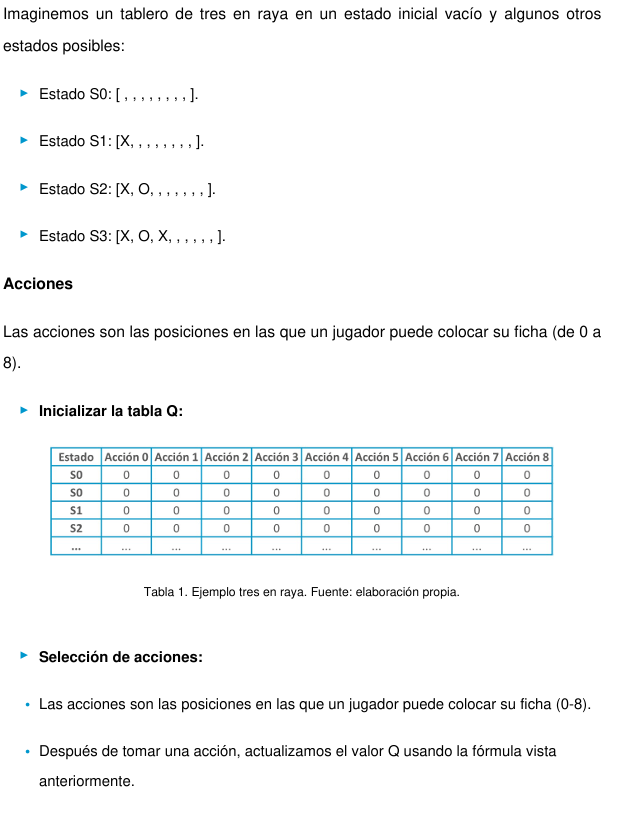
\includegraphics[width=\linewidth]{imagenes/tresenraya1.png}
        \label{fig:tresenraya1}
    \end{minipage}
    \hfill
    \begin{minipage}{0.48\linewidth}
        \centering
        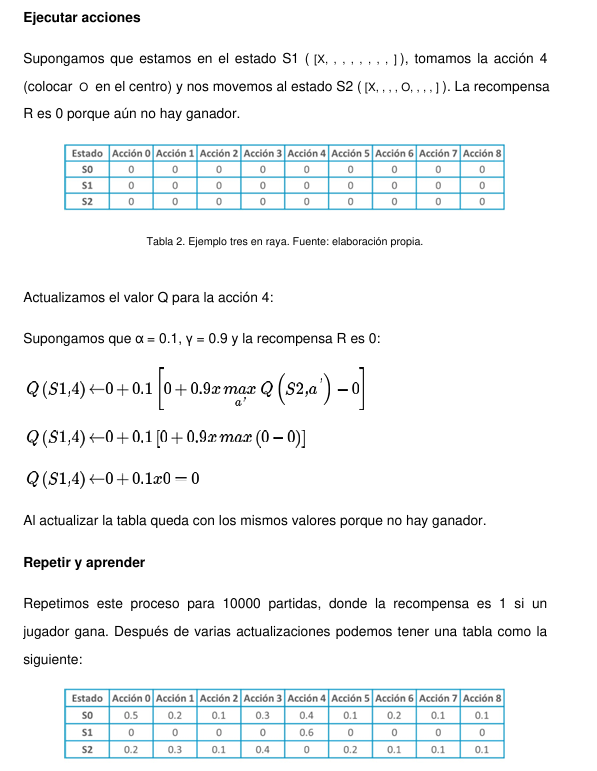
\includegraphics[width=\linewidth]{imagenes/tresenraya2.png}
        \label{fig:tresenraya2}
    \end{minipage}
\end{figure}

\newpage

\section{Deep Q-Network (DQN)}

El algoritmo Q-learning es efectivo en entornos simples, pero resulta inviable cuando el número de estados y acciones crece considerablemente, ya que no es práctico usar una tabla Q. Para superar esta limitación, se desarrolló el \textbf{Deep Q-Network (DQN)}, que combina Q-learning con redes neuronales profundas para aproximar la función Q y manejar grandes espacios de estados.

DQN utiliza dos redes neuronales:
\begin{itemize}
    \item \textbf{Red principal:} parametrizada por $\theta$, estima los valores Q del estado $s$ y acción $a$ actuales, es decir, $Q(s, a; \theta)$.
    \item \textbf{Red objetivo:} parametrizada por $\theta'$, tiene la misma arquitectura que la principal y se utiliza para calcular los valores Q objetivo del siguiente estado $s'$ y acción $a'$. Sus parámetros se actualizan periódicamente copiando los de la red principal.
\end{itemize}

La red Q predice los valores para cada acción y se elige aquella con el valor más alto. El objetivo es minimizar la pérdida del error cuadrático medio (MSE) entre los valores Q predichos y los valores Q objetivo:
\[
Loss = \left(Q_{\text{objetivo}} - Q_{\text{Predicha}}\right)^2
\]

Los valores Q objetivo se calculan usando la ecuación de Bellman:
\[
Q_{\text{target}} = R + \gamma \max(Q_{\text{next}})
\]
donde $R$ es la recompensa obtenida y $Q_{\text{next}}$ es el valor máximo estimado por la red objetivo para el siguiente estado.

Al igual que en Q-learning, la política óptima $\pi$ consiste en seleccionar en cada estado la acción con el mayor valor Q estimado y continuar este proceso para maximizar la recompensa esperada a lo largo del tiempo.

\begin{center}
\begin{tikzpicture}[
  node distance=1.5cm and 2.5cm,
  every node/.style={draw, rounded corners, align=center, minimum width=3.5cm, minimum height=1.2cm, font=\normalsize},
  arrow/.style={-Stealth, thick}
]
\node (estado) {Estado};
\node (redq) [right=of estado] {Red neuronal Q};
\node (valores) [right=of redq, draw=none, align=left, font=\normalsize] {
  Valor Q acción 1\\
  Valor Q acción 2\\
  \vdots\\
  Valor Q acción n
};

\draw[arrow] (estado) -- (redq);
\draw[arrow] (redq) -- (valores);
\end{tikzpicture}
\end{center}





\section{Algoritmo REINFORCE}

El \textbf{algoritmo REINFORCE} (``REward Increment = Nonnegative Factor $\times$ Offset Reinforcement $\times$ Characteristic Eligibility'') es una técnica clásica de aprendizaje por refuerzo basada en el método de gradiente de políticas.

REINFORCE aprende directamente una \textbf{política}: una función que mapea estados a probabilidades de acciones. La política se parametriza (por ejemplo, con una red neuronal) y se ajusta iterativamente mediante el cálculo de gradientes y ascenso de gradiente para maximizar la recompensa acumulada esperada.

El agente interactúa con el entorno siguiendo su política actual, obteniendo una secuencia de recompensas. El retorno acumulado desde el tiempo $t$ se calcula como:
\[
R_t = r_t + \gamma r_{t+1} + \gamma^2 r_{t+2} + \cdots + \gamma^{T-t-1} r_{T-1}
\]
donde $r_t$ es la recompensa en el paso $t$, $\gamma$ es el factor de descuento y $T$ es el último paso del episodio.

El gradiente para actualizar los parámetros de la política es:
\[
\Delta\theta = \alpha \nabla_\theta \log \pi_\theta(a_t|s_t) R_t
\]
donde $\alpha$ es la tasa de aprendizaje, $\nabla_\theta \log \pi_\theta(a_t|s_t)$ es el gradiente logarítmico de la política y $R_t$ la recompensa acumulada.

\subsection*{Conceptos clave}
\begin{itemize}
    \item \textbf{Política ($\pi$):} Estrategia que sigue el agente para tomar decisiones, parametrizada como $\pi^\theta(a|s)$.
    \item \textbf{Función de recompensa acumulada ($R$):} Suma de recompensas recibidas a lo largo de un episodio.
    \item \textbf{Gradiente de la política:} Se utiliza para ajustar los parámetros de la política en la dirección que maximiza la recompensa esperada.
\end{itemize}


\section{Proximal Policy Optimization (PPO)}

OpenAI publicó un artículo denominado \textit{Algoritmos de optimización de políticas próximas} (PPO) como una nueva familia de métodos de gradiente de políticas. PPO es conocido por ser robusto y eficiente, y se utiliza para entrenar agentes en entornos donde las decisiones se toman en base a políticas, es decir, reglas que determinan las acciones a tomar en cada estado del entorno.

\subsection{Tres puntos principales}
\begin{itemize}
    \item \textbf{PPO alterna} entre el muestreo de datos a través de la interacción con el entorno y la optimización de una función objetivo-sustituta mediante un ascenso de gradiente estocástico.
    \item A diferencia de los métodos de gradiente de políticas estándar, que realizan una actualización de gradiente por muestra de datos, PPO introduce una función objetivo novedosa que permite múltiples épocas de actualizaciones en minibatch.
    \item PPO ofrece algunos de los beneficios de la optimización de políticas de región confiable (TRPO), pero es más simple de implementar, más general y tiene una mejor complejidad de muestra empíricamente.
\end{itemize}

\subsection{Conceptos clave en este algoritmo}
\begin{itemize}
    \item \textbf{Función de valor} ($V$): mide lo bueno que es estar en un estado en particular.
    \item \textbf{Ratio de probabilidad} ($r_t(\theta)$): es el ratio entre la nueva política y la política antigua. Es clave en PPO para medir el cambio de la política:
    \[
    r_t(\theta) = \frac{\pi_\theta(a_t|s_t)}{\pi_{\text{old}}(a_t|s_t)}
    \]
    \item \textbf{Clip objetivo}: se introduce una función objetivo que limita (clip) los ratios de probabilidad para mantener actualizaciones de política dentro de un rango razonable.
\end{itemize}

La función objetivo es:
\[
L^{\text{CLIP}}(\theta) = \mathbb{E}_t \left[ \min \left( r_t(\theta) \hat{A}_t, \; \text{clip}\left(r_t(\theta), 1 - \epsilon, 1 + \epsilon \right)\hat{A}_t \right) \right]
\]
donde $\hat{A}_t$ es la ventaja estimada y $\epsilon$ es un hiperparámetro que controla cuánto puede cambiar el ratio de probabilidad.

\subsection{Entrenamiento del algoritmo PPO}
El algoritmo PPO se entrena de la siguiente manera:
\begin{enumerate}
    \item Recolección de datos, ejecutando la política actual para recolectar datos de interacción del agente con el entorno.
    \item Estimación de la ventaja $\hat{A}_t$ para cada acción tomada.
    \item Actualización de la política utilizando $L^{\text{CLIP}}(\theta)$ para asegurar que las actualizaciones no sean demasiado grandes.
    \item Este proceso se repite, ajustando la política gradualmente para mejorar el desempeño del agente.
\end{enumerate}





\section{Comparativa de técnicas aprendizaje por refuerzo}


\begin{figure}[ht]
    \centering
    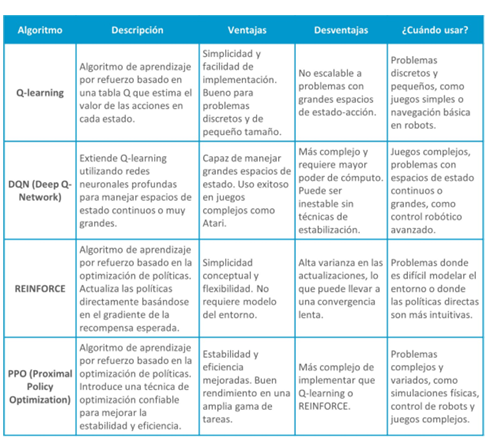
\includegraphics[width=1\linewidth]{imagenes/comparativa-q-learning.png}
    \label{fig:comparativa-q-learning}
\end{figure}